\chapter{Numerical Techniques}\label{chap:3}
In this chapter, I will present the numerical methods relevant to this thesis.
The incompressible Navier-Stokes equations describe the time- and spatial-varying velocity field and pressure field.
One of the foundations of solving partial differential equations begin with the method of weighted residuals. 

%%%%%%%%%%%%%%%%%%%%%%%%%%%%%%%%%%
% 3.1 METHOD OF WEIGHTED RESIDUALS
%%%%%%%%%%%%%%%%%%%%%%%%%%%%%%%%%%

\section{Method of weighted residuals}
We discuss the method of weighted residuals which provides a mathematical framework for approximating the solutions of partial differential equations.
We first  consider a generic linear partial differential equation as,
\begin{equation}\label{eq:linear_operator}
    \mathbf{L}[u(x)] = 0, \quad x \in \Omega
\end{equation}
where $\mathbf{L}$ refers to a spatial (linear) differential operator subjected to some boundary conditions within the domain, $\Omega$ while $u(x)$ refers to the solution.
Typical examples of spatial differential operators are the Laplace, Poisson or Helmholtz operators.
In seeking the solution, $u(x)$, we assume that it could be approximated by a finite number of $N$ basis (or expansion) functions, $\Phi(x)$, 
\begin{equation}\label{eq:approximate}
    u(x) \approx u^\delta(x) = \sum_{i=0}^{N-1} \hat{u}_i \Phi_i(x),
\end{equation}
where $u^\delta(x)$ refers to the approximate solution of $u(x)$, comprising of a linear combination of the product between the $i^{th}$ basis coefficient, $\hat{u}_i$, and a basis function $\Phi_i(x)$, that is defined within $\Omega$.
Since $u^\delta(x)$ is an approximate solution of equation \eqref{eq:helmholtz}, we expect a non-zero difference (or `error') between the exact solution, $u(x)$, and $u^\delta(x)$, known as the residual, $R$, given as,
\begin{equation}\label{eq:residual}
    \mathbf{L}[u^\delta(x)] = R[u^\delta(x)].
\end{equation}
The residual depends on the approximate solution $u^\delta(x)$, and is non-zero, varying within $\Omega$.
In other words, equation \eqref{eq:helmholtz} might not be satisfied everywhere in $\Omega$. 
We need to place restrictions on the residual, such that it $R \rightarrow 0$, and the approximate solution approaches the exact solution, $u^\delta(x) \rightarrow u(x)$.
The method of residuals allow us to place a restriction on $R$ is by using $N$ weight (or test) functions, $v_j(x)$, such that it is orthogonal with the residual,
\begin{equation}\label{eq:weightinnerresidual}
    (v_j(x), R[u^\delta(x)]) = 0, \quad j = 0, ..., N-1.
\end{equation}
where $(\, \cdot \, , \, \cdot \,)$ refers to an inner-product, a measure of orthogonality between functions defined as,
\begin{equation}\label{eq:inner-product}
       (f, g) = \int_\Omega f(x) g(x) dx.
\end{equation}
By setting the inner-product to $0$, equation \eqref{eq:weightinnerresidual} becomes a system of $N$ ordinary differential equations, where the basis coefficients, $\hat{u}_i$, could be determined as we shall see later.
The choice of weight function defines the class of projection methods, and the common projection methods are shown in table \ref{tab:weightFunction}.
It is worth noting that the method of weighted residuals describes the projection method, and does not specify the type of basis functions employed.
The choice of projection method, and basis expansions will have different solution convergence properties, i.e. how does the residual decay as the number of basis expansions increases?
By considering Fourier basis expansions, one can expect exponential convergence, desirable for an efficient representation of turbulent dynamics.
% Certain mathematical properties such as spectral convergence as desired in the case of Galerkin projection using Fourier expansions, 
% The choice of \emph{trial} functions used in \emph{nektar++} will be elaborated in Section \ref{sec:modifiedBasis}.
% the method of weighted residuals is only restrictive to the weight
% Table \ref{tab:weightFunction} shows the different forms of weight functions and its corresponding numerical method.
\renewcommand{\arraystretch}{1.5} % Default value: 1
\begin{table}[h]
    \centering
        \begin{tabular}{cc}
            Weight functions & Projection method \\
            \hline
            $v_j(x) = \delta(x-x_j)$ & Collocation \\
            $v_j(x) =\left\{\begin{array}{ll}
                1 & \mbox{if } x \in \Omega_j\\
                0 & \mbox{if } x \notin \Omega_j \\
           \end{array}\right. $& Finite-Volume \\
            $v_j(x) = \phi_j$& Galerkin \\
            $v_j(x) = \frac{\partial R}{\partial \hat{u}_j}$ & Least-squares \\
            \hline
        \end{tabular}
        \caption{Examples of weight functions and projection methods}
    \label{tab:weightFunction}
\end{table}
% For instance, for $v_j = \delta(x-x_j)$, the numerical method becomes the \emph{collocation} method where the differential equation is satisfied on discrete points $x_j$.
% The type of restriction on the residual is implemented through the choice of \emph{test} function, $v_j$.
\section{Galerkin Projection}
The Galerkin projection is a remain as a projection method in finite elements, where the weight functions, $v(x)$, are chosen to be the same as the basis functions, $\Phi(x)$.
We will elaborate on what defines being the `same' later.
To demostrate the Galerkin projection method, we consider that the spatial (linear) differential operator in equation \eqref{eq:linear_operator} as a 1D Helmholtz equation,
\begin{subequations}\label{eq:helmholtz}
    \begin{equation}
        \mathbf{L}[u(x)] \equiv \frac{\partial^2 u(x)}{\partial x^2} - \lambda u(x) - f(x) = 0, \quad x \in \Omega := [0, l]
    \end{equation}
    \begin{equation}
        u(0) = g_D, \quad \frac{\partial u}{\partial x}\Big|_{x=l} = g_{N}.
    \end{equation}
\end{subequations}
where $\lambda$ is a real positive constant, $f(x)$ is the forcing function, and $\Omega$ the spatial domain bounded between $0$ and $l$. 
% $ hh u(x), \lambda, f, \Omega$ refers to the linear (spatial) differential operator, solution to the diffential equation, a real positive constant, forcing function and the spatial domain bounded between 0 and $l$, respectively.
To ensure that problem is well-posed, we impose both Dirichlet and Neumann boundary conditions, corresponding to $g_D$ and $g_N$, at $x = 0$ and $x = l$, respectively.
% In order for the problem to be well-posed, we impose both Dirichlet and Neumann, boundary conditions corresponding to $g_D$ and $g_N$ at $x= 0 $ and $x=l$, respectively.
Equation \ref{eq:helmholtz} is said to be written in the \textit{strong} or \textit{classical} form.

Next, we begin to construct the weak form by taking the inner product of the Helmholtz equation with a weight function, which satisfies the homogeneous Dirichlet boundary conditions by definition, and require this inner product to vanish, that is,
\begin{equation}\label{eq:helmholtz_inner}
    (w, \mathbf{L}[u(x)]) = \int_0^l w\left[\frac{\partial^2 u(x)}{\partial x^2} - \lambda u(x) + f(x)\right] \mathrm{d}x =  0.
\end{equation}
This step is equivalent to applying the method of weighted residuals, where $u(x)$ could refer to the approximate solution, $u^\delta(x)$. 
We perform integration by parts next, 
\begin{equation}\label{eq:weak_form}
    \underbrace{\int_0^l \frac{\partial v}{\partial x}\frac{\partial u}{\partial x} \mathrm{d}x + \int_0^l \lambda v u \mathrm{d}x}_{a(v,u)}= \underbrace{\int_0^l v f \mathrm{d}x + \left[ v \frac{\partial u}{\partial x} \right]_0^l}_{f(v)}.
\end{equation}
This equation is typically referred to as the weak form of equation \eqref{eq:helmholtz}.
In compact notation, we define the bilinear and linear forms as,
\begin{subequations}
    \begin{equation}
        a(v,u) = f(v),
    \end{equation}
\end{subequations}
where $a(v,u)$ and $f(v)$ are typically refered to as the strain energy and forcing function in structural mechanics, assumed to remain finite.
To ensure this, we restrict the choice of solutions $u(x)$ to lie in the functional solution space, $\mathcal{U}$, defined as
\begin{equation}
    \mathcal{U} := \{ u | u \in H^1, u(0) = g_D \},
\end{equation}
where $u \in H^1$ contains functions of $u$ in the Sobolev space such that the Dirichlet condition $u(0) = g_D$ is statisfied and the sum of square integral of $u$ and its first derivatives, $\frac{\partial u}{\partial x}$ remains bounded,
\begin{equation}
    \int_\Omega \left ( u^2 + \left(\frac{\partial u}{\partial x} \right)^2 \right) \mathrm{d}\Omega < \infty.
\end{equation}
We consider functions up to the first-derivatives since the it is the highest-order derivative in equation \eqref{eq:helmholtz_inner}.
Similarly, the functional space of weight functions, $\mathcal{V}$, is defined as,
\begin{equation}
    \mathcal{V} := \{ v | v \in H^1, v(0) = 0 \},
\end{equation}
where $v \in H^1$ are functions whose values and first derivatives are square-integrable and satisfy a homogeneous Dirichlet boundary condition at $x = 0$.
The generalised weak form is therefore finding $u(x) \in \mathcal{X}$, such that
\begin{equation}
    a(v,u) = f(v), \quad \forall v \in \mathcal{W}.
\end{equation}
This formulation is still infinite-dimensional, as the function space $\mathcal{U}, \mathcal{W}$ contain infinitely many functions.
To obtain an approximate solution, $u^\delta(x)$, we restrict ourselves to finite-dimensional subspaces, $\mathcal{U}^\delta \subset \mathcal{U}$, and $\mathcal{V}^\delta \subset \mathcal{V}$.
The problem is then to find $u^\delta \in \mathcal{U}^\delta$, such that
\begin{equation}
    a(v^\delta, u^\delta) = f(v^\delta), \quad v^\delta \in \mathcal{V}^\delta
\end{equation}
Here, both $u^\delta \in \mathcal{U}^\delta$ and $v^\delta \in \mathcal{V}^\delta$ do not lie in same subspace, necessary for the standard Galerkin projection procedure where they should lie in the same subspace.
To overcome this, we lift the solution $u^\delta$ into two parts,
\begin{equation}
    u^\delta = u^\mathcal{H} + u^\mathcal{D}.
\end{equation}
where $u^\mathcal{H} \in \mathcal{V}^\delta$ satisfies the homogeneous Dirichlet condition, lying in the same subsapce as $w^\delta \in \mathcal{V}^\delta$, and $u^\mathcal{D} \in \mathcal{U}^\delta$ satisfies the Dirichlet boundary conditions $u^\mathcal{D}(0) = g_D$.
Substituting this decomposition, the standard Galerkin projection methos is to search for the solution $u^\mathcal{H} \in \mathcal{V}^\delta$ such that,
\begin{equation}\label{eq:standard_galerkin}
    a(v^\delta, u^\mathcal{H}) = f(v^\delta) - a(v^\delta, u^\mathcal{D}).
\end{equation}
We have briefly described the mathematical framework for approximating a solution to the linear (spatial) partial differential operator.
In the following, we will expand on the type of basis and weight functions , $\Phi(x)$, specifically, using the spectral/\emph{hp} element method, and describe essential differential and integral operations performed numerically, equation \eqref{eq:standard_galerkin} reduces to a system of linear equations.

%%%%%%%%%%%%%%%%%%%%%%
% SPECTRAL/HP ELEMENTS
%%%%%%%%%%%%%%%%%%%%%%

\section{Spectral/\emph{hp} element methods}
% To represent the spatially-dependent velocity and pressure fields, spatial discretisation is performed using the spectral/\emph{hp} element method.
% Other popular methods of spatial discretisation found in literature are the finite-difference methods, and finite-volume methods.
% The spectral/{hp} element method (SEM) is related to the Galerkin method in which the type of \emph{trial} function used. The spectral/\emph{hp} element method combines 2 traditional numerical methods, namely, 
The spectral/\emph{hp} element method is a spatial discretisation technique in which the solution domain is partitioned into a set of non-overlapping (finite) elements with size $h$, each consisting of a linear combination of continuous polynomial functions of up to order $P$. 
% represented by a polynomial of up to order $p$.
% which leverages the advantages of offering geometric flexibility by decomposing the global domain into a set of non-overlapping (finite) elements of size $h$, each consisting of a linear combination of continuous polynomial functions of up to order $p$.
It leverages the geometric flexibility of classical finite-element methods, allowing for the representation of complex engineering geometries, and the exponential (spectral) convergence properties of classical spectral methods, where the solution error decreases exponentially.
% The Spectral/\emph{hp} element method leverages the advantages of both methods - geometric flexibility and spectral covergence.
% The spectral/\emph{hp} method uses a series of high-order polynomials (Lagrange/Legendre) within each element.
Suppose we consider $P+1$ linearly independent polynomials spanning the polynomial space of $\mathcal{P}_P$, the error of a smooth solution with element size of $h$ and polynomial order $P$ has the property of \citep{karniadakis_spectralhp_2005}, 
\begin{equation}\label{eq:error_convergence}
    ||u(x) - u^{\delta}(x)|| \leq Ch^P||u(x)|| \approx \mathcal{O}(h^P).
\end{equation}
where $C$ is some constant.
Equation \ref{eq:error_convergence} implies that the error decreases linearly with $h$, and exponentially with $P$.

% % It offers the flexibility of offering refinements in either $h$ or $p$, or both.
% \begin{enumerate}
%     \item Finite elements:
%         \subitem The finite element method decomposes the global domain into a set of non-overlapping subdomains (finite elements), represented by linear shape functions. In a 1D domain, the size of each element is given by $h$ and the approximate solution should covergence as $h$ is decreased - also known as \emph{h}-refinement. The flexibility of domain decomposition allows for complex engineering geometries to be represented. 
%     \item Spectral method:
%         \subitem The spectral method performs a global discretisation of the domain. The domain is represented by a linear combination of global continuous functions, such as the Fourier series. Spectral methods benefit from the property of \emph{spectral convergence}, where the solution error decreases by $\mathcal{O}(c^{-N})$, where $c$ is some constant $0 \leq c \leq 1$ and $N$ is the number of polynomials (\cite{trefethen_2000}). In other words, as the number of functions is increased, the error decreases exponentially.
% \end{enumerate}

%%%%%%%%%%%%%%%%%%
% DOMAIN PARTITION
%%%%%%%%%%%%%%%%%%
\subsection{Domain partition}
We consider a one-dimensional domain, $\Omega$ defined earlier, and seek to decompose it into a set of $N_{el}$ elements, where $\Omega^e$, refers to the elemental partitions with $1 \geq e \geq N_{el}$ such that they meet at their boundaries,
\begin{equation}
    \Omega = \bigcup_{e = 1}^{N_{el}} \Omega^e, \quad \text{where} \; \bigcap_{e=1}^{N_{el}} \Omega^e = \emptyset
\end{equation}
where $e^{th}$ element is defined as,
\begin{equation}
    \Omega^e = \{x | x_{e-1} \geq x \geq x_e \},
\end{equation}
Each element it then represented by a linear combination, $\phi(x)$, where $x$ is referred to the \emph{global} domain.

%%%%%%%%%%%%%%%%%%%
% STANDARD ELEMENTS
%%%%%%%%%%%%%%%%%%%
\subsection{Standard Elements}
In general, we can expect non-uniform elements so it is useful to define a \emph{standard} element,
\begin{equation}
    \Omega_{set} := \{ \xi | -1 \geq \xi \geq 1 \},
\end{equation}
where $\Omega_{st}$ refers to the standard element, defined over local coordinates, $\xi \in [-1, 1]$.
By considering formulations using the standard elements, the formulations of basis expansions, differential and integration operations can be performed in local coordinates, $\xi$, before mapping the results back to the global domain, $x$.
\begin{figure}[h]
    \centering
    \includegraphics[width=\textwidth]{NumericalTechniques/Figures/standard_element.pdf}
    \caption{A spectral/\emph{hp} element representation of a 1D continuous function, $u(x)$, deomposed into four non-overlapping finite elements, each containing a linear combination of three local expansion bases.}
    \label{fig:standard_element}
\end{figure}
We can map the standard element into any arbitrary global coordinates based on a linear mapping $\chi^e:\Omega_{st} \rightarrow \Omega$,
\begin{equation}
    x = \chi^e(\xi) = \frac{1-\xi}{2} x_e + \frac{1 + \xi}{2}x_{e+1}, \quad \xi \in \Omega_{st}
\end{equation}
which has an analytical inverse, $(\chi^e)^{-1}(x)$,
\begin{equation}
    \xi = (\chi^e)^{-1}(x) = 2 \frac{x - x_{e-1}}{x_e - x_{e-1}} - 1, \quad x \in \Omega_{st}.
\end{equation}
In each standard element, we can represent the solution by using a linear combination of local expansion basis, $\phi(\xi)$,
\begin{equation}
    \phi_0(\xi) = \frac{1 - \xi}{2}, \quad \phi_1(\xi) = (1 + \xi)(1 - \xi), \quad \phi_2(\xi) =  \frac{1 + \xi}{2},
\end{equation}
where $\phi_0, \phi_2$ denotes a linear local expansion basis with $P = 1$, while $\phi_1$ is a quadratic local expansion basis with $P=2$. 
The approximate solution is now represented as,
\begin{equation}
    u^\delta(x) = \sum_{i=0}^{N-1}\hat{u}_i\Phi_i(x) = \sum_{e=0}^{N_{el}-1}\sum_{i=0}^P \hat{u}_i^{e}\phi^e_i(\chi^e(\xi)).
\end{equation}
where $\hat{u}_i^e, N_{el}$ refers to the local expansion basis coefficients the number of elements.
Consequentially, $u^\delta(x)$ now lie within $\mathcal{X}^\delta$.
\begin{equation}
    \mathcal{X}^\delta := \left\{ u^\delta \,\middle|\, u^\delta \in H^1,\ u^\delta(\chi^e(\xi)) \in \text{span}\{\phi_0, \phi_1, \phi_2\},\ e = 1, 2, 3, 4 \right\}
\end{equation}
Figure \ref{fig:standard_element} summarises the domain partition based on standard elements.

%%%%%%%%%%%%%%%%%%%%
% ASSEMBLY FUNCTIONS
%%%%%%%%%%%%%%%%%%%%

\subsection{Assembly process}
As we represent our solution using local expansion basis within standard elements, their solution across the elemental boundaries may become discontinuous.
In the approach of continuous Galerkin projection methods, we enforce our solution to be $C^0$ continuous across the elemental boundaries.
In other words, the neighbouring linear interior elements must meet at the boundaries, such that the local expansion coefficients are constrained by,
\begin{equation}
    \hat{u}^{e-1}_P = \hat{u}^e_0.
\end{equation}
This constrain enforeced by consider a mapping between the (global) expansion coefficients, and local expansion coefficients, 
% Due to the constraint described above, we need a mathematical process which maps the local coefficients to the global coefficients.
% To fulfil this description, we introduce a vector of global coefficients, $\mathbf{\hat{u}}_g$, and local coefficients $\mathbf{\hat{u}}_l$, and a linear map $\mathbf{A}$, given as,
% In this case, we introduce the definition of global modes given as,
% \begin{equation}
%     u^\delta(x) = \sum_{i=0}^{N_{dof}-1} \hat{u}_i \Phi_i(x) = \sum_{e=1}^{N_{el}}\sum_{i=0}^P \hat{u}_i^{e}\phi^e_i(\chi^e(\xi)).
% \end{equation}
% where $\Phi_i(x)$ refers to global modes, that is defined in the entire domain.
\begin{subequations}

    \begin{equation}
        \mathbf{\hat{u}}_l = \mathbf{A} \mathbf{\hat{u}}_g   
    \end{equation}
    \text{with,}
    \begin{equation}
        \mathbf{\hat{u}}_l = 
        \begin{bmatrix}
            \hat{u}_0^1  \\
            \hat{u}_1^1  \\
            \hat{u}_2^1  \\
            \hat{u}_0^2  \\
            \hat{u}_1^2  \\
            \hat{u}_2^2  \\
            \hat{u}_1^3  \\
            \hat{u}_2^3  \\
            \hat{u}_3^3  \\
        \end{bmatrix}
        \quad
        \mathbf{A} = 
        \begin{bmatrix}
            1 & 0 & 0 & 0 & 0 & 0 & 0\\
            0 & 1 & 0 & 0 & 0 & 0 & 0\\
            0 & 0 & 1 & 0 & 0 & 0 & 0\\
            0 & 0 & 1 & 0 & 0 & 0 & 0\\
            0 & 0 & 0 & 1 & 0 & 0 & 0\\
            0 & 0 & 0 & 0 & 1 & 0 & 0\\
            0 & 0 & 0 & 0 & 1 & 0 & 0\\
            0 & 0 & 0 & 0 & 0 & 1 & 0\\
            0 & 0 & 0 & 0 & 0 & 0 & 1\\
        \end{bmatrix}
        ,
        \quad 
        \mathbf{\hat{u}}_g
        \begin{bmatrix}
            \hat{u}_0  \\
            \hat{u}_1  \\
            \hat{u}_3  \\
            \hat{u}_4  \\
            \hat{u}_5  \\
            \hat{u}_6  \\
            \hat{u}_7 
        \end{bmatrix}
    \end{equation}
\end{subequations}
where $\mathbf{\hat{u}}_l, \mathbf{\hat{u}}_g, \mathbf{A} \in \mathbb{R}^{N_l, N_g}$ refers to the vector of local, global expansion and scatter matrix, and $N_l = N_{el} \times (P + 1)$ refers to the total local degrees of freedom while $N_g = N_l - (N_{el} - 1)$, the global degrees of freedom.
Notably, matrix $\mathbf{A}$ `scatters' the global degrees of freedom to local degrees of freedom.
In the spectral/\textit{hp} approach, we typically define local expansion basis, and perform integration and differentiation operation in standard element.
After doing so, we need to assemble the operations from the standard element to the global domain by using $\mathbf{A}^T$, is known as an assembly operation, assembling local degrees of freedom to global degrees of freedom.
For instance, we wish to perform integration in the domain $\Omega$, 
\begin{equation}
    \mathbf{I}_g[j] = (\Phi_j(x), u^\delta(x)),
\end{equation}
which equivalent to performing integration using local expansion basis within standard elements, and assembling in the global space by using $\mathbf{A}^T$,
\begin{subequations}
    \begin{equation}
        \mathbf{I}_g = \mathbf{A}^T \mathbf{I}_l
    \end{equation}
    \begin{equation}
    \mathbf{I}_g =  
    \begin{bmatrix}
        \mathbf{I}_0 \\
        \vdots \\
        \mathbf{I}_{N_g-1}
    \end{bmatrix}
    ,
    \quad 
    \mathbf{I}_l =  
    \begin{bmatrix}
        \mathbf{I}^0 \\
        \vdots \\
        \mathbf{I}^{N_{el}-1}
    \end{bmatrix}
    ,\quad \text{where} \quad
    \mathbf{I}^e =  
    \begin{bmatrix}
        \int_{-1}^1 \phi_0^e(\xi) u(\chi^e)\frac{\mathrm{d} \chi^e}{\mathrm{d} \xi}\, \mathrm{d}\xi \\
        \vdots \\
        \int_{-1}^1 \phi_{P-1}^e(\xi) u(\chi^e)\frac{\mathrm{d} \chi^e}{\mathrm{d} \xi}\, \mathrm{d}\xi
    \end{bmatrix}
    \end{equation}
\end{subequations}
and $\mathbf{I}_g, \mathbf{I}_l, \mathbf{I}^e$ refer to the integration operations perform in global, local and elemental space.

% \begin{equation}
%     \mathbf{I}_g[j] = (\Phi_j(x), u^\delta(x)) = \int_\Omega \Phi_j(x) \, \sum_{i=0}^P\sum_{e=0}^{N_{el} -1} \hat{u}_i^e\phi_i^e(\chi^e(\xi)) \, \mathrm{d} x
% \end{equation}



%%%%%%%%%%%%%%%%%
% BASIS FUNCTIONS
%%%%%%%%%%%%%%%%%

\subsection{Expansion functions}
Here, we discuss the expansion functions of $\phi(\xi)$, where in general could be categorised into \emph{modal} (hierarchical) expansions or \emph{nodal} expansions.
% Modal expansions
\subsubsection{Modal expansions}
The most common modal employed in Nektar++ are the Jacobi polynomials, denoted by $P_p^{\alpha,\beta}(x)$, which represent a family of polynomial solutions to the Sturm-Liouville problem wihin, $x \in [-1, 1]$.
The Legendre polynomials are a special case of Jacobi polynomials, $L_n(\xi) = P_n^{0,0}(\xi)$ with $\alpha = \beta = 1$.
% The \emph{trial} functions $\phi_p$ (or basis expansions) used in spectral/\emph{hp} method consist of \emph{boundary} and \emph{interior} modes.
% \emph{Interior} modes are defined to be zero on all boundaries, and non-zero within the boundary, satisfying homogeneous boundary conditions.
% \emph{Boundary} modes take on non-zero values on the boundary, satisfying non-homogeneous boundary conditions and providing $C^0$ continuity between elements (\cite{karniadakis_2005spectral}).
Within the Nektar++ framework, it is common to use the \emph{modified} basis based on Jacobi polynomials, ${P}_p^{\alpha,\beta}(\xi)$ which are modified with linear elements as
% are used as the \emph{trial} functions. Using $\alpha=1$, $\beta=1$, and linear basis functions as \emph{boundary} modes, the modified Jacobi polynomials are,
\renewcommand{\arraystretch}{1.25} % Default value: 1
\begin{equation}\label{eq:modifiedJacobi}
    \phi_p(\xi) = \psi_p(\xi) = \left\{
            \begin{array}{ll}
                \frac{1-\xi}{2} & \mbox{for } p=P\\
                \frac{1-\xi}{2}\frac{1+\xi}{2}{P}_{P-1}^{1,1}(\xi) & \mbox{for } P \geq 2 \\
                \frac{1+\xi}{2} & \mbox{for } p=P,
           \end{array}\right.
\end{equation}
where $P$ denotes the highest polynomial order. Figure \ref{fig:Modifiedbasis} shows the modified Jacobi polynomials for $p \in [0, 5]$ described by equation \ref{eq:modifiedJacobi}. The boundary modes are $\psi_0$ and $\psi_5$ while the rest are boundary modes.
\begin{figure}[h]
    \centering
        \includegraphics[width=\textwidth]{NumericalTechniques/Figures/modifiedBasis.pdf}
        \caption{Two-dimensional and one-dimension modified basis, $\psi_p(\xi_1)$ and $\psi_q(\xi_2)$, $P = [0, 4].$}
        \label{fig:Modifiedbasis}
\end{figure}

% Nodal expansions
\subsubsection{Nodal expansions}
A popular nodal expansions are the Lagrange polynomials, common used in the spectral \textit{element} codes such as Semtex and Nek5000.
The Lagrange polynomials are given as
\begin{equation}
    \phi_p(\xi) = h_p(\xi) = \frac{\prod_{q = 0, q \neq p}^P (\xi - \xi_q)}{\prod_{q = 0, q \neq p}^P (\xi_p - \xi_q)}
\end{equation}
The Lagrange polynomials are particular attractive as it has a unit value at $\xi_q$ and zero everywhere else,
\begin{equation}
    h_p(\xi_q) = \delta_{pq}.
\end{equation}
Typically, the zeros are located using the zeros of the Gauss-Lobatto polynomials where the zeros are defined using
\begin{equation}
    \phi_p(\xi) \rightarrow h_p(\xi) = \begin{cases} 1, & \quad \xi = \xi_p, \\ \frac{(\xi^2 -1)[P_{Q-1}^{\alpha,\beta}(\xi)]'}{(Q-1)(Q+\alpha+\beta)P_{Q-1}^{\alpha,\beta}(\xi_j)(\xi - \xi_j)}, & \quad \text{otherwise.} \end{cases}
\end{equation}

\begin{figure}[h]
    \centering
    \includegraphics[width=\textwidth]{NumericalTechniques/Figures/Lagrange.pdf}
    \caption{Two-dimensional and one-dimension Lagrange basis, $h_p(\xi_1)$ and $h_q(\xi_2)$, $P = [0, 4].$}
    \label{fig:Lagrangebasis}
\end{figure}
Figure \ref{fig:Lagrangebasis} presents nodal expansions based on two-dimensional and one-dimensional Lagrange polynomials, $h_p(\xi_1), h_q(\xi_2)$ respectively.

The modified basis and Lagrange exhibits stark differences.

%%%%%%%%%%%%%%%%%%%%%%%%%%%
% NUMERICAL Integration
%%%%%%%%%%%%%%%%%%%%%%%%%%%
\subsection{Numerical integration}
In the Galerkin formulation, we perform integration routinely.
Suppose we want to approximate the integral of a smooth function in a standard element numerically,
\begin{equation}
    \int_{-1}^1 u(\xi) \; \mathrm{d}\xi = \sum_{i=0}^{Q-1} w_i u(\xi_i) + R(u),
\end{equation}
where $Q, w_i, \xi_i, R(u)$ refers to the quadrature points, integration weights and zeros (or abscissae) and the integral of the error.
By evaluating the integral, how are we able to minimise the integral error, $R(u)$, with the least number of quadrature points, $Q$, at some weights and zeros.
If $u(\xi)$ is of polynomial order $P$, we can expect we might need at least $P+1$ equipspaced points to accurately represent the function and evalute its integral, a rather inefficient method.
Gaussain quadrature is allow us to approximate an integral of a function of order $P$ with far lesser thatn $P+1$ points, as we shall see later.
The three generic types of Gaussian quadrature rules are known as: Gauss, Gauss-Radau and Gauss-Lobatto.
The main difference between the three methods are in the treatment of the zeros, where Gauss quadrature uses zeros without the end points $\xi = \pm 1$.
Gauss-Radau quadrature either select one of the end points, usually at $\xi = -1$, and Gauss-Lobatto consider the end points.
We will only focus on describing the Gauss-Lobatto quadrature rules and the zeros of Jacobi polynomials known as the Gauss-Lobatto-Jacobi quadrature rules given as,
\begin{subequations}
    \begin{equation}
        \xi_i^{\alpha,\beta} = \begin{cases}
            -1 \quad & i = 0, \\
            \xi_{i-1,Q-2}^{\alpha+1, \beta+1} \quad & i = 1, ..., Q-2,\\
            1, \quad & i = Q-1,
        \end{cases}
    \end{equation}
    \begin{equation}
        w_i^{\alpha,\beta} = \begin{cases}
            (\beta + 1) C_{0,Q-2}^{\alpha, \beta}, \quad & i = 0, \\
            C_{i,Q-2}^{\alpha,\beta}, \quad & i = 1, ..., Q-2, \\
            (\alpha + 1) C^{\alpha,\beta}_{Q-1,Q-2}, \quad & i = Q - 1,
        \end{cases}
    \end{equation}
    \begin{equation}
        C_{i,Q-2}^{\alpha, \beta} = \frac{2^{\alpha+\beta+1}\Gamma(\alpha+Q)\Gamma(\beta+Q)}{(Q-1)(Q-1)!\Gamma(\alpha+\beta+Q+1)[P_{Q-1}^{\alpha,\beta}(\xi_i)]^2}
    \end{equation}
\end{subequations}
where $w_i^{\alpha,\beta}, \xi_i^{\alpha,\beta}$ are the zeros and weights of the Gauss-Lobatto-Jacobi quadrature rules, and $\Gamma$ refers to the Gamma function.
By using these conventions, we can obtain an exact integral of a continuous function, $u(\xi)$ of polynomial $P$, with at least $Q \geq (P+3)/2$ quadrature points.

%%%%%%%%%%%%%%%%%%%%%%%%%%%
% NUMERICAL DIFFERENTIATION
%%%%%%%%%%%%%%%%%%%%%%%%%%%

\subsection{Numerical differentiation}
In the same fashion as Gaussian quadrature, we want to numerical differentiate efficiently, a crucial step in the weak formulation of the Helmholtz equations.
Suppose that we want to differentiate in $x$ using local coordinates given as,
\begin{equation}
    \frac{\mathrm{d} u^\delta(\xi)}{\mathrm{d} x} = \frac{\mathrm{d} u ^\delta(\xi)}{\mathrm{d} \xi}\frac{\mathrm{d} \xi}{\mathrm{d} x} = \sum_{p = 0}^P \hat{u}_p \frac{\mathrm{d} \phi_p(\xi)}{\mathrm{d}\xi}\frac{\mathrm{d}\xi}{\mathrm{d} x},
\end{equation}
where $\mathrm{d}\xi/\mathrm{d}x$ is simply the Jacobian and the main step in differentiation is in evaluting $\mathrm{d} \phi_p(\xi) / \mathrm{d} \xi$.
Now suppose that we express the solution of polynomial order $P$ with Lagrange polynomials, the derivative of the solution commutes,
\begin{equation}
    \frac{\mathrm{d} u(\xi)}{\mathrm{d} \xi} = \sum_{i=0}^{Q-1} u(\xi_i) \frac{\mathrm{d}}{\mathrm{d} \xi} h_i(\xi),
\end{equation}
where we only require the derivative to be evaluted at the nodal points, resulting in a derivative matrix of,
\begin{equation}
    D_{ij} = \frac{\mathrm{d} h_j (\xi)}{\mathrm{d} \xi}\Big|_{\xi = \xi_i}, 
\end{equation}
and the derivative of $u(\xi)$ is simply,
\begin{equation}
    \frac{\mathrm{d} u(\xi)}{\mathrm{d} \xi} \Big|_ {\xi = \xi_i} = \sum_{j=0}^{Q-1} D_{ij}\hat{u}_j.
\end{equation}
A general representation of the differential operator can be presented as
\begin{equation}
    D_{ij} = \begin{cases} 
    \frac{p'_Q(\xi_i)}{p'_Q(\xi_j)} \frac{1}{\xi_i - \xi_j}, \quad & i \neq j, \\
    \frac{p''_Q(\xi_i)}{2p'_Q(\xi_i)}, \quad & i = j.
\end{cases}
\end{equation}
where $p'_Q(\xi), p''_Q(\xi)$ are specific restricted to the quadrature used.
For the Gauss-Lobatto-Jacobi quadrature rules used here, these forms could be found in Appendix C.2 in \cite{karniadakis_spectralhp_2005}.

%%%%%%%%%%%%%%%
% EXAMPLE IN 1D
%%%%%%%%%%%%%%%

\subsection{Example in 1D}
We have outlined the basic formulation of spectral/\emph{hp} element methods in $1D$ and we will describe its solution procedure, where we start from the weak-form of the Helmholtz equation and convert it into a system of linear equations, amenable to be solved with standard numerical linear algebra techniques.
We describe the solution steps as follows,
\subsubsection{1. Performing numerical differentiation and integration in the standard region}
\begin{equation}
    \lambda \underbrace{\int_{-1}^1 v^\delta u^\mathcal{H} \, \mathrm{d}\xi}_{\mathbf{M}^e\mathbf{\hat{u}}^e} + \underbrace{\int_{-1}^1 \frac{\partial v^\delta}{\partial \xi}\frac{\partial u^\mathcal{H}}{\partial \xi} \mathrm{d}\xi}_{\mathbf{L}^e \mathbf{\hat{u}}^e} = \underbrace{\int_{-1}^1 v^\delta f \mathrm{d}\xi}_{\mathbf{\hat{f}}^e}
\end{equation}
\subsubsection{Elemental mass operator}
Here we introduce the elemental mass operator given as $\mathbf{M}^e$,
\begin{align}
    \int_{-1}^1 \sum_{i = 0}^{P}\hat{v}^e_i\phi^e_i(\xi) \sum_{i = 0}^{P}\hat{u}^e_i\phi^e_i(\xi) \, \mathrm{d}\xi &= \sum_{q=0}^{Q} \left[ \sum_{i = 0}^{P}\hat{v}_i^e\phi_i^e(\xi_q) \sum_{i = 0}^{P}\hat{u}^e_i\phi_i^e(\xi_q) \right]w_q^e\\ \nonumber
 & = (\mathbf{\hat{v}}^e)^T (\mathbf{B}^e)^T \mathbf{W}^e \mathbf{B}^e \mathbf{\hat{u}}^e \\ \nonumber
& = \mathbf{\hat{v}}^T \mathbf{M}^e \mathbf{\hat{u}}^e
\end{align}
where $\mathbf{M}^e = (\mathbf{B}^e)^T \mathbf{W} \mathbf{B}^e$ refers to the elementral mass matrix, while $\mathbf{B}^e \in \mathbb{R}^{Q-1,P}$ and $\mathbf{W}^e\in \mathbb{R}^{Q-1,Q-1}$ refers to the elemental basis and weight matrices, a diagonal matrix consisting of integration weights, $w_q^e$, respectively,
\begin{equation}
    \mathbf{B}^e = 
    % \begin{bmatrix}
    %     \begin{bmatrix}
    %         | \\
    %         \mathbf{\phi_0} \\
    %         |
    %     \end{bmatrix}
    %     &
    %     \cdots
    %     &
    %     \begin{bmatrix}
    %         | \\
    %         \mathbf{\phi_P} \\
    %         | \\
    %     \end{bmatrix}
    % \end{bmatrix}
    % =
    \begin{bmatrix}
        \phi_0(\xi_0) & \cdots & \phi_P(\xi_0) \\
        \vdots & \ddots & \vdots \\
        \phi_0(\xi_Q) & \cdots & \phi_P(\xi_Q) \\
    \end{bmatrix}
    ,
    \quad
    \mathbf{W}^e = 
    \begin{bmatrix}
        w_0^e &  & 0 \\
         & \ddots &  \\
        0 & & w_Q^e  
    \end{bmatrix}
\end{equation}
\subsubsection{Elemental laplacian matrices}
Now we consider, convert the product of two first-derivatives in to matrix form,
\begin{align}
    \int_{-1}^1 \sum_{i = 0}^{P}\hat{v}^e_i\frac{\mathrm{d} \phi^e_i}{\mathrm{d} \xi} \sum_{i = 0}^{P}\hat{u}^e_i\frac{\mathrm{d} \phi^e_i}{\mathrm{d} \xi} \, \mathrm{d}\xi &= \sum_{q=0}^{Q} \left[ \sum_{i = 0}^{P}\hat{v}^e_i{D}_{qi}^e\phi^e_i(\xi_q) \sum_{i = 0}^{P}\hat{u}^e_i{D}^e_{qi}\phi_i^e(\xi_q) \right]w_q^e\\ \nonumber
& = \mathbf{\hat{v}}^T (\mathbf{B}^e)^T (\mathbf{D}^e)^T \mathbf{W}^e \mathbf{D}^e \mathbf{B}^e \mathbf{\hat{u}}^e \\ \nonumber
& = \mathbf{\hat{v}}^T \mathbf{L}^e \mathbf{\hat{u}}^e
\end{align}
where $\mathbf{L}^e = (\mathbf{B}^e)^T(\mathbf{D}^e)^T  \mathbf{W} \mathbf{D}^e \mathbf{B}^e$ refers to the elementral Laplacian matrix.
\subsubsection{Forcing vector}
Lastly, we consider the right-hand side,
\begin{align}
    \int_{-1}^1 \sum_{i = 0}^P \hat{v}_i^e\phi_i^e(\xi) f^e(\xi) \, \mathrm{d}\xi & = \sum_{q=0}^P \sum_{i = 0}^P \hat{v}_i^e \phi_i^e (\xi_q) f^e(\xi_q) w_q^e, \\ \nonumber
                                                                                & = \mathbf{\hat{v}}^T (\mathbf{B}^e)^T\mathbf{W}^e \mathbf{f}^e \\ \nonumber
                                                                                & = \mathbf{\hat{v}}^T \mathbf{\hat{f}}^e,
\end{align}
where $\mathbf{\hat{f}}^e$, is referred to the elemental forcing vector.
As we consider all of the matrices, the Helmholtz equations in elemental form is simply solving for,
\begin{equation}
    \left[ \lambda \mathbf{M}^e + \mathbf{L}^e \right] \mathbf{\hat{u}}^e = \mathbf{\hat{f}}^e.
\end{equation}
If we considered bolting the elements together and the boundary conditions,
\begin{equation}
    \lambda 
    \underbrace{
    \begin{bmatrix}
        \mathbf{M}^0+\mathbf{L}^0 &  & \mathbf{0} \\
         & \ddots & \\
        \mathbf{0} &  & \mathbf{M}^{N_{el} - 1} + \mathbf{L}^{N_{el}-1}\\
\end{bmatrix}}_{\mathbf{M}_l + \mathbf{L}_l}
\underbrace{
    \begin{bmatrix}
        \mathbf{\hat{u}}^0 \\
        \vdots  \\
        \mathbf{\hat{u}}^{N_{el}-1}
\end{bmatrix}}_{\mathbf{\hat{u}}_l}
     = 
    \begin{underbrace}{
    \begin{bmatrix}
        \mathbf{\hat{f}}^0 \\
        \vdots  \\
        \mathbf{\hat{f}}^{N_{el}-1}
\end{bmatrix}}_{\mathbf{\hat{f}}_l}
    + 
    \underbrace{
    \begin{bmatrix}
        \mathbf{L}^0g_D \\
        \vdots  \\
        \mathbf{0}
\end{bmatrix}}_{\mathbf{g}_D}
    +
    \underbrace{
    \begin{bmatrix}
        \mathbf{0} \\
        \vdots  \\
        g_N
\end{bmatrix}}_{\mathbf{g}_N},
\end{equation}
where $\mathbf{M}_l, \mathbf{L}_l, \mathbf{\hat{u}}_l, \mathbf{\hat{f}}_l, \mathbf{g}_D, \mathbf{g}_N$ refers to the local mass matrix, local laplacian matrix, and vector of local expansion coefficients , Dirichlet and Neumann boundary conditions.
Finally, we can assemble them using the assembly matrix,
\begin{equation}
    \mathbf{A}^T ( \lambda \mathbf{M}_l + \mathbf{L}_l) \mathbf{A} \mathbf{\hat{u}}_g = \mathbf{A}^T(\mathbf{\hat{f}}^l + \mathbf{g}_D + \mathbf{g}_N),
\end{equation}


%%%%%%%%%%%%%%%%%%%%%%%%%%%%%%%%%%%%%
% TECHNIQUES FOR SOLVING NS EQUATIONS
%%%%%%%%%%%%%%%%%%%%%%%%%%%%%%%%%%%%%

\section{Numerical techniques for solving the Navier-Stokes equations}
\subsection{Velocity Correction Scheme}
While methods for temporal and spatial discretisation have been discussed, it is not possible to apply these techniques in a straight-forward manner to the incompressible Navier-Stokes equations. This is because of the unique role of the pressure field which ensures that the time-dependent velocity field is divergence-free. However, the velocity and the pressure fields form a coupled-system through the continuity and momentum equations which requires the solution of both fields simultaneously. In general, there are 3 ways to deal with velocity-pressure coupling: (1) Coupled methods (\emph{Uzawa} method), (2) Change of variables (streamfunction-vorticity formulation) and (3) Splitting methods which decouples velocity and pressure. The velocity correction scheme (VCS) (\cite{karniadakis_1991}), a type of splitting method, decouples the velocity field from the pressure field used in \emph{nektar++} will be discussed in this section. The velocity correction scheme is a stiffly-stable time-integration (IMEX) scheme which treats the nonlinear terms (advection) explicitly and linear terms (pressure gradient and diffusion) implicitly.
The VCS will be demonstrated through a worked example. The incompressible Navier-Stokes equations with unit density, constant density and viscosity is written as,
\begin{equation}\label{eq:navierStokes}
    \frac{\partial \mathbf{u}}{\partial t} = \mathrm{\mathbf{N}(\mathbf{u})} - \nabla p +  \nu \mathrm{\mathbf{L}}(\mathbf{u}), \qquad \nabla \cdot \mathbf{u},
\end{equation}
where $\mathbf{u},\; p,\; \rho,\; \nu$ refers to the fluid's velocity, pressure, density and kinematic viscosity respectively. The convection and diffusion terms are conveniently written as nonlinear and linear functions,
\begin{equation}
    \mathrm{\mathbf{N}}(\mathbf{u}) \equiv - (\mathbf{u} \cdot \nabla)\mathbf{u} = -\frac{1}{2}\left[(\mathbf{u} \cdot \nabla )\mathbf{u} + \nabla\cdot(\mathbf{u}\mathbf{u})\right], \qquad \mathrm{\mathbf{L}}(\mathbf{u}) \equiv \nabla^2 \mathbf{u}.
\end{equation}
The nonlinear terms are written in the skew-symmetric to minimise aliasing errors (\cite{karniadakis_1991}). The first step in the scheme is to time integrate the nonlinear terms explicitly,
\begin{equation}\label{eq:firstStep}
    \frac{\mathbf{\hat{u}} - \sum_{q=0}^{J_e-1} \alpha_{q} \mathbf{u}^{n-q}}{\Delta t} = \sum_{q=0}^{J_e-1} \beta_q \mathrm{\mathbf{N}}(\mathbf{u}^{n-q}),
\end{equation}
where $\mathbf{\hat{u}}$ is the first intermediate velocity field, $J_e$ denotes the order of the explicit scheme, superscript $n$ denotes the solution at the $n^{th}$ time-step and $\alpha_q,\; \beta_q$ refers to constant related to the IMEX schemes. Next, the second intermediate velocity field $\hat{\hat{\mathbf{u}}}$ is obtained from the gradient of the pressure field at $n+1$,
\begin{equation}\label{eq:secondStep}
    \frac{\mathbf{\hat{\hat{u}}} - \mathbf{\hat{u}}}{\Delta t} = -\nabla p^{n+1}.
\end{equation}
However, the pressure field at time-step $n+1$ is not known. Taking the divergence of equation \ref{eq:secondStep}, and assuming that $\hat{\hat{\mathbf{u}}}$ is divergence-free, the Poisson equation for pressure is given as,
\begin{equation}\label{eq:pressurePoisson}
    \nabla^2 p^{n+1} = \nabla \cdot \left(\frac{\mathbf{\hat{u}}}{\Delta t}\right).
\end{equation}
with the following boundary condition,
\begin{equation}\label{eq:pressureBC}
\frac{\partial p^{n+1}}{\partial n} = \mathbf{n} \cdot \left(\frac{\mathbf{\hat{\hat{u}}} - \mathbf{\hat{u}}}{\Delta t}\right)
\end{equation}
However, this boundary condition often suffer from splitting errors and may lead to wrong solutions (\cite{karniadakis_1991}). To rectify this, the boundary condition is directly obtain by taking normal dot product with \ref{eq:navierStokes} and evaluated explicity (\cite{alessandro_phd_2013}),
\begin{equation}\label{eq:modifiedpressureBC}
    \frac{\partial p^{n+1}}{\partial t} = -\sum_{q=0}^{J_e-1} \beta_q \left[ \frac{1}{\Delta t} \mathbf{u}^{n-q} + \nu (\nabla \times \omega^{n-q}) + (\mathbf{u}^{n-q} \cdot \nabla)\mathbf{u}^{n-q} \right] \cdot \mathbf{n}.
\end{equation}
where $\omega = \nabla \times \mathbf{u}$, $J_e$ is the order for the explicit scheme, $\beta_q$ is the coefficient related to the time-integration scheme. We obtain the pressure field at time-step $n+1$ by solving the pressure Poisson equation (\ref{eq:pressurePoisson}) with the modified boundary conditions (\ref{eq:modifiedpressureBC}). Then, the second intermediate velocity field $\hat{\hat{\mathbf{u}}}$ is obtained from equation \ref{eq:secondStep}. Finally, the velocity field at $n+1$ is obtain from the final step of the scheme by solving
\begin{equation}\label{eq:thirdStep}
    \frac{\gamma_0\mathbf{u}^{n+1} - \hat{\hat{\mathbf{u}}}}{\Delta t} = \nu \sum_{q=0}^{J_i-1} \beta_q \mathrm{\mathbf{L}}(\mathbf{u}^{n+1-q}), \qquad \mathbf{u}^{n+1}|_{\delta\Omega} = g_D
\end{equation}
where $J_i$ denotes the order of the implicit scheme, $\gamma_0,\; \beta_q$ are coefficients related to the stiffly stable time-integration scheme and $\mathbf{u}^{n+1}$ satisfies the Dirichlet boundary conditions. Table \ref{tab:stiffyStableCoefficients} shows the coefficients of stiffly-stable time-integration schemes (\cite{alessandro_phd_2013}).
\renewcommand{\arraystretch}{1.5} % Default value: 1
\begin{table}[h]
    \centering
        \begin{tabular}{c|c|c}
            test & $1^{st}$ order & $2^{nd}$ order \\
            \hline
            $\gamma_0$ & 1 & 3/2 \\
            $\beta_0$ & 1 & 2 \\
            $\beta_1$ & 0 & -1 \\
            $\alpha_0$ & 0 & -1/2 \\
            $\alpha_1$ & 0 & 0 
        \end{tabular}
        \caption{Stiffly-stable splitting scheme coefficients}
    \label{tab:stiffyStableCoefficients}
\end{table}

%%%%%%%%%%%%%%%%%%%%%%%%%%%%%%%%%%%%%
% FOURIER SPECTRAL/HP ELEMENT METHODS
%%%%%%%%%%%%%%%%%%%%%%%%%%%%%%%%%%%%%

\subsection{Fourier spectral/\emph{hp} modes}
The Fourier spectral/\emph{hp} element method uses a combination of Fourier expansions and spectral/\emph{hp} element method to discretise the spatial domain. In a turbulent channel flow, the Fourier expansions are used to represent the periodic streamwise and cross stream directions, while the spectral/\emph{hp} elements are used to discretise the wall-normal direction. Within the \emph{nektar++} framekwork, the Fourier spectral/\emph{hp} element method (also known as a Quasi-3D approach), can be implemented either with 2D spectral/\emph{hp} elements and 1D Fourier expansions (3DH1D) or 1D spectral/\emph{hp} elements and 2D Fourier expansions (3DH2D). In this work, the 2D spectral/\emph{hp} elements with 1D Fourier expansions are used to discretise the cross stream plane and streamwise flow respectively. The use of 2D spectral/\emph{hp} elements in the cross stream plane is necessary to represent the riblet geometry (\cite{chu_1993}). The time- and spatially-varying velocity and pressure in the cross stream planes are approximated as a finite sum of 2D modified Jacobi polynomials up to the $P^{th}$-order,
\renewcommand{\arraystretch}{1.} % Default value: 1
\begin{equation}\label{eq:crossStream}
    \begin{bmatrix}
        \mathbf{u}^\delta(y,z,t) \\
        p^\delta(y,z,t)
    \end{bmatrix}
    =
    \sum_{p=0}^P \sum_{q=0}^P \psi_p(y) \psi_q(z)
    \begin{bmatrix}
         \hat{\mathbf{u}}_{p,q}(t) \\
         \hat{p}_{p,q}(t)
    \end{bmatrix}
\end{equation}
where $\hat{\mathbf{u}}_{p,q}(t)$ and $\hat{p}_{p,q}(t)$ are the time-varying coefficients. Extending equation \ref{eq:crossStream} to include the streamwise direction represented by Fourier expansions,
\begin{equation}\label{eq:fourierSpectral}
    \begin{bmatrix}
        \mathbf{u}^\delta(x,y,z,t) \\
        p^\delta(x,y,z,t)
    \end{bmatrix}
    =
    \sum_{k=0}^{N-1} \sum_{p=0}^P \sum_{q=0}^P \psi_p(y) \psi_q(z) e^{ik\alpha x}
    \begin{bmatrix}
         \hat{\mathbf{u}}_{p,q,k}(t) \\
         \hat{p}_{p,q,k}(t)
    \end{bmatrix}
    =
    \sum_{k=0}^{N-1} e^{ik\alpha x} \begin{bmatrix}
        \mathbf{u}_k(y,z,t) \\ p_k(y,z,t)
    \end{bmatrix}
\end{equation}
where $\alpha = \frac{2\pi}{L_x}$ is the streamwise wavenumber, $L_x$ is the streamwise domain length and $N$ refers to the number of Fourier expansions. Substituting equation \ref{eq:fourierSpectral} into the Navier-Stokes equations and taking the Fourier transform (equivalently to the Galerkin projection with respect to Fourier expansion as a test function) yields $N$-systems of equations,
\begin{equation}
    \frac{\partial \mathbf{u}_k}{\partial t} = - \tilde{\nabla}_k p_k + \nu(\nabla^2_{y,z} - k^2\alpha^2)\mathbf{u}_k - \widehat{\left[(\mathbf{u} \cdot \nabla) \mathbf{u}\right]}_k, \qquad \tilde{\nabla}\mathbf{u}_k = 0
\end{equation}
where, $\tilde{\nabla} = (ik\alpha, \frac{\partial}{\partial y}, \frac{\partial}{\partial z})$, $\nabla_{y,z}^2 = (\frac{\partial^2}{\partial y^2}, \frac{\partial^2}{\partial z^2})$ and $\widehat{\left[(\mathbf{u} \cdot \nabla) \mathbf{u} \right]_k}$ refers to the Fourier-transformed of the $k^{th}$ nonlinear term.

\subsection{Enforcing constant flow rate}
Due to the enforced periodicity in the streamwise $z$ direction via Fourier expansions, a pressure drop cannot be prescribed to drive the flow for $Re > 0$ scenarios.
To sustain the flow, we use a Green's function approach \citep{chu1992parallel} to impose a constant flow rate,
\begin{equation}
    W_b = Q(\mathbf{u})=\frac{1}{2L_x h}\int_{x,y} \mathbf{u} \; \mathrm{d}x\mathrm{d}z,
\end{equation}
where $W_b$ and $Q(\cdot)$ refer to the desired flow rate and flow rate operator.
A correction velocity, $\mathbf{u}_{corr}$, is obtained by solving the linear Stokes equation with unit forcing once and is stored for reuse.
At the end of every time-step, the final velocity field, $\mathbf{u}$, is then updated by adding this correction velocity to the homogeneous velocity obtained from the velocity correction scheme,
\begin{equation}
    \mathbf{u} = \mathbf{u}_h + \gamma \mathbf{u}_{corr}, 
\end{equation}
where $\gamma$ defined as,
\begin{equation}
    \gamma = \frac{ W_b - Q(\mathbf{u}_h)}{Q(\mathbf{u}_{corr})},
\end{equation}
is adjusted to satisfy the desired flow rate, $W_b$.
The flow rate, $W_b$, is related to the laminar centreline velocity $W_c = 3/2 W_b$, which defines the Reynolds number, $Re = W_c h / \nu$.
For more details on the numerical method, the reader is referred to \cite{hossain2021spectral}.

\section{Stability analysis of the Navier-Stokes equations}
\subsection{Linear Stability analysis}
\subsection{Edge state computations}




% The choice of \emph{test} function is also commonly known as projection methods, i.e projecting (taking the inner product) the residual onto the \emph{test} functions.
% Usually, the weight functions are selected 
% An approximate solution has $K+1$ unknowns ($\hat{u}_0, ...,\hat{u}_K$), hence, it is natural to impose $K+1$ restrictions on the residual to form a determined system and the type of restriction defines the numerical method. 
% The goal is to choose appropriate basis expansions and weights such that the approximate solution approaches the exact solution where $R[u^\delta(x)] \rightarrow 0$.
% We premultiply equation \eqref{eq:residual} with a suitable weight function, $w(x)$, and take the inner-product defined as,
% he solution is an approximate one, equation \eqref{ref:helmholtz}, id no
% In the context fluid mechanics, the Fourier series can be used to represent isotropic turbulence with homogenenous (periodic) boundary conditions.
% In a channel flow, Fourier series are used in the homogenenous streamwise ad spanwise directions while Chebyshev or Legendre polynomials are used in the wall-normal direction.

Consider equation \ref{eq:infiniteExpansions} to be a solution of a 1-dimensional Poisson equation, bounded by the domain $\Omega \in [x_a, x_b]$,
Next, we consider that the expansion functions, $\phi_i(x)$, belongs to an element of a Hilbert space, with a suitable inner-product.

The mathematical framework begins by first assuming that the solution, $u(x)$, is an element of a Hilbert space, $\mathcal{H}$ with a suitable inner-product $(\cdot, \cdot)$ and norm $|| \cdot ||$.
For 
SEMs belong to a general class of methods known as the method of weighted residual, a generic method for approximating a solution of a differential equation. The method of weighted residual will be described with a worked example as follows. Consider that the solution of a differential equation $u(x)$ can be represented as an infinite sum of \emph{trial} \citep{karniadakis_spectralhp_2005}. functions (also known as basis functions, expansion functions, mode shapes).
\begin{equation}\label{eq:infiniteExpansions}
\end{equation}
where $\phi_i(x)$ are the \emph{trial} functions and $\hat{u}_i$ are the trial function coefficients to be determined.
with the appropriate boundary conditions, and $\mathbb{L}$ refers to a linear differential operator. Note that equation \ref{eq:infiniteExpansions} exactly satisfies the differential equation of \ref{eq:linearOperator} i.e $\mathbb{L}u(x)- f(x) = 0$. The exact solution would require a computation of infinite basis coefficients $\hat{u}$ which is practically infeasible. Therefore, an approximate solution $u^\delta(x)$ is sought after by truncating an infinite number of basis expansions to a finite number,
\begin{equation}\label{eq:truncatedExpansions}
    u(x) \approx u^\delta (x) = \sum_{i=0}^{K}\hat{u_i}\phi_i(x),
\end{equation}
where there is a finite number of $K$ basis expansions. The approximate solution does not satisfy \ref{eq:linearOperator} exactly, leading to an 'error' known as a residual,
\begin{equation}
    R(u^\delta(x)) = \mathbb{L}u^\delta(x) - f(x)
\end{equation}

The method of weighted residual is a general method that allows for various types the restriction to be implemented. The method "nullifies" the residual by equating the inner product with a \emph{test} function, $v_j(x)$ (also known as a weight function - hence the name 'weighted residual') to zero,
\begin{equation}\label{eq:residual}
    (v_j(x), R(u^\delta(x))) = \int_{x_a}^{x_b} v_j\,R(u^\delta(x))\; \mathrm{d}x = 0, \qquad j = 0,...,K.
\end{equation}

% \subsection{Galerkin methods}
Galerkin methods are commonly found in finite/spectral element solvers, used in \emph{nektar++}. The Galerkin method belongs to a general class of weighted residual methods that assumes the \emph{trial} functions take on the same form as the \emph{test} functions (Table \ref{tab:weightFunction}). To describe the method, a worked example is illustrated. The Galerkin method is appplied to solve the Poisson equation \ref{eq:linearOperator} with the following boundary conditions,
\begin{equation}\label{eq:boundaryConditions}
    B^- = g^- \quad \textrm{at} \quad x = x_a, \qquad B^+ = g^+ \quad \textrm{at} \quad x = x_b
\end{equation}
where $B^-$, $B^+$ are the boundary conditions which could be either Dirichlet, Neumann or Robin conditions. Equation \ref{eq:linearOperator} and \ref{eq:boundaryConditions} together forms a boundary value problem and is said to be in the \emph{strong} \footnote{\emph{strong} loosely mean that the trial functions are required to be both $C^0$ and $C^1$ continuous} form. The Galerkin method assumes that the trial functions $\phi_i(x)$ satisfies equation \ref{eq:linearOperator} with homogeneous boundary conditions,
\begin{equation}
    \phi_i(x_a) = \phi_i(x_b) = 0.
\end{equation}
Next, the solution $u(x)$ is decomposed into a linear combination of $\tilde{u}(x)$ and $u^H(x)$,
\begin{equation}
    u(x) = \tilde{u}(x) + u^H(x),
\end{equation}
where $\tilde{u}(x)$ is any function that satisfy the boundary conditions assosciated with equation \ref{eq:boundaryConditions} and $u^H(x)$ is the homogeneous solution that satisfies the homogeneous boundary conditions - $B_H^-(x_a) = B_H^+(x_b) = 0$. The resulting problem for $u^H(x)$ becomes
\begin{equation}\label{eq:linearHomogeneous}
    \mathbb{L}u^H(x) - h(x) = 0, \qquad x_a \leq x \leq x_b,
\end{equation}
where $h =  f(x) - \mathbb{L}\tilde{u}(x)$. It is worth noting that the steps thus simply mathematical, and no approximation have been made. The solutions of $u(x) = \tilde{u}(x) - u^H(x)$ represented by an infinite expansions (equation \ref{eq:infiniteExpansions}) are exact. Next, the homogeneous solution  $u^H(x)$ can be approximated by a finite expansion of \emph{trial} functions,
\begin{equation}\label{eq:homogeneousCoefficients}
    u^H(x) \approx u^{H,\delta} (x) = \sum_{i=0} ^ K \hat{u}^{H,\delta}_i\phi_i(x),
\end{equation}
where $\hat{u}^{H,\delta}_i$ are the coefficients to be determined. Since $\phi_i(x)$ satisfies the homogeneous boundary conditions, $\hat{u}^{H, \delta}_i$ can take on any values and $u^{H, \delta}(x)$ will still satisfy the homogeneous boundary conditions. Substituing the approximate solution of $u^{H,\delta}(x)$ into equation \ref{eq:linearHomogeneous}, and applying the method of weighted resiudal,
\begin{equation}\label{eq:galerkinResidual}
    (R(u^{H,\delta}), v_j(x)) = \int_{x_a}^{x_b} \left(\mathbb{L}u^{H,\delta}(x) - h(x) \right) v_j(x) \; \mathrm{d}x = 0, \qquad j=0, ..., K,
\end{equation}
where $v_j(x)$ is some \emph{test} function and there are $K+1$ finite expansions. In the Galerkin method (or Bubnov-Galerkin), the weight function $v_j(x)$ takes on the same form as the trial functions $\phi_j(x)$ (Table \ref{tab:weightFunction}). In other words, the differential equation is satisfied when projected on the \emph{test/trial} functions. Substituting equation \ref{eq:homogeneousCoefficients} into the residual equation \ref{eq:galerkinResidual} and applying $v_j(x) = \phi_j(x)$,
\begin{equation}\label{eq:generalisedGalerkin}
    \sum_{i=0}^{K} \hat{u}^{H,\delta}_i \int_{x_a}^{x_b} \mathbb{L}\phi_i\phi_j \; \mathrm{d}x = \int_{x_a}^{x_b} \left(f(x) - \mathbb{L}\tilde{u}(x) \right) \phi_j \; \mathrm{d}x, \qquad j = 0, .., K
\end{equation}
Equation \ref{eq:generalisedGalerkin} furnishes a system of $K+1$ linear equations with $K+1$ unknowns i.e $\{\hat{u}^{H,\delta}_0,....,\hat{u}^{H,\delta}_K\}$. Applying integration by parts to equation \ref{eq:generalisedGalerkin}, the equation reduces to,
\begin{equation}
    \sum_{i=0}^K \hat{u}_i^{H,\delta} \left[\int_{x_a}^{x_b} \frac{\partial \phi_j}{\partial x}\frac{\partial \phi_i}{\partial x} + \lambda \phi_j\phi_i \; \mathrm{d}x\right] = - \int_{x_a}^{x_b} \frac{\partial \tilde{u}}{\partial x}\frac{\partial \phi_j}{\partial x} + (\lambda\tilde{u} + f(x))\phi_j \; \mathrm{d}x,
\end{equation}
which is known as the \emph{weak}\footnote{\emph{trial} functions are only required to be $C^0$ continuous} form. The boundary conditions of the \emph{weak} form naturally appears in the right-hand side of equation \ref{eq:systemOfLinear}, which makes it convenient to implement. Equation \ref{eq:generalisedGalerkin} can be re-written in matrix form,
\renewcommand{\arraystretch}{1.25} % Default value: 1
\begin{equation}\label{eq:systemOfLinear}
    \begin{split}
    &\begin{bmatrix}
        \int_{x_a}^{x_b} \frac{\partial \phi_0}{\partial x}\frac{\partial \phi_0}{\partial x} + \lambda\phi_0\phi_0 \; \mathrm{d}x & \hdots & 
        \int_{x_a}^{x_b} \frac{\partial \phi_0}{\partial x} \frac{\partial \phi_K}{\partial x} + \lambda\phi_0\phi_K \; \mathrm{d}x \\
        \vdots & \ddots & \vdots \\
        \int_{x_a}^{x_b} \frac{\partial \phi_K}{\partial x}\frac{\partial \phi_0}{\partial x} + \lambda\phi_0\phi_0 \; \mathrm{d}x & \hdots & 
        \int_{x_a}^{x_b} \frac{\partial \phi_K}{\partial x} \frac{\partial \phi_K}{\partial x} + \lambda\phi_0\phi_K \; \mathrm{d}x \\
    \end{bmatrix}
    \begin{bmatrix}
        \hat{u}_0^{H,\delta} \\ \vdots \\ \hat{u}_K^{H, \delta}
    \end{bmatrix}
    = \\
    &\begin{bmatrix}
        -\int_{x_a}^{x_b} \frac{\partial \tilde{u}}{\partial x} \frac{\partial \phi_0}{\partial x} + (\lambda \tilde{u} + f(x))\phi_0 \; \mathrm{d}x \\ 
        \vdots \\ 
        -\int_{x_a}^{x_b} \frac{\partial \tilde{u}}{\partial x} \frac{\partial \phi_K}{\partial x} + (\lambda \tilde{u} + f(x))\phi_K \; \mathrm{d}x \\ 
    \end{bmatrix}
    \end{split}
\end{equation}
where $\mathbf{\hat{u}}^{H,\delta} = [\hat{u}_0^{H,\delta}, ..., \hat{u}_K^{H, \delta}]$ is determined by solving the system of linear equations. 

%%%%%%%%%%%%%%%%%%%%%%%%%%%%%%%%%%
% 3.2 Spectral/hp element methods
%%%%%%%%%%%%%%%%%%%%%%%%%%%%%%%%%%

\section{The Spectral/{hp} element methods}
To represent the spatially-dependent velocity and pressure fields, spatial discretisation is performed using the spectral/\emph{hp} element method.
Other popular methods of spatial discretisation found in literature are the finite-difference methods, and finite-volume methods.
The spectral/{hp} element method (SEM) is related to the Galerkin method in which the type of \emph{trial} function used. The spectral/\emph{hp} element method combines 2 traditional numerical methods, namely, 
\begin{enumerate}
    \item Finite elements:
        \subitem The finite element method decomposes the global domain into a set of non-overlapping subdomains (finite elements), represented by linear shape functions. In a 1D domain, the size of each element is given by $h$ and the approximate solution should covergence as $h$ is decreased - also known as \emph{h}-refinement. The flexibility of domain decomposition allows for complex engineering geometries to be represented. 
    \item Spectral method:
        \subitem The spectral method performs a global discretisation of the domain. The domain is represented by a linear combination of global continuous functions, such as the Fourier series. Spectral methods benefit from the property of \emph{spectral convergence}, where the solution error decreases by $\mathcal{O}(c^{-N})$, where $c$ is some constant $0 \leq c \leq 1$ and $N$ is the number of polynomials (\cite{trefethen_2000}). In other words, as the number of functions is increased, the error decreases exponentially.
\end{enumerate}
The Spectral/\emph{hp} element method leverages the advantages of both methods - geometric flexibility and spectral covergence. The spectral/\emph{hp} method uses a series of high-order polynomials (Lagrange/Legendre) within each element. Considering each element consists of $P+1$ linearly independent polynomials (where $P$ refers to the highest polynomial order) spanning the polynomial space of $\mathcal{P}_P$, the error of a smooth solution with mesh-size $h$ and polynomial order $P$ has the property of (\cite{karniadakis_2005spectral}),
\begin{equation}\label{eq:errorConvergence}
    ||u(x) - u^{\delta}(x)|| \leq Ch^P||u(x)|| \approx \mathcal{O}(h^P).
\end{equation}
Equation \ref{eq:errorConvergence} implies that the error decreases as the $h$ is decrease (mesh refinement) or as $P$ is increased using higher-order polynomials.

% \subsection{Polynomial expansions in SEM}\label{sec:modifiedBasis}
%%%%%%%%%%%%%%%%%%%%%%%%%%%%%%
% 3.3 TEMPORAL DISCRETISATIONS
%%%%%%%%%%%%%%%%%%%%%%%%%%%%%%

% \section{Temporal Discretisation}\label{sec:temporalDiscret}
% The velocity and pressure fields obtained from the Navier-Stokes equations are time dependent. A separate class of numerical methods used for temporal discretisation will be covered in this section. Temporal discretisation methods, used to solve initial value problems (IVPs) can be broadly categorised into two schemes:
% 
% \begin{enumerate}
%     \item Multi-stage schemes that advance the solution from the $n^{th}$ to $n^{th}+1$ time-step through a number of intermediate stages which are not solutions at the previous time-steps. The class of Runge-Kutta schemes is an example of multi-staged schemes. In general, multi-stage schemes are typically computationally intensive as extra intermediate steps are required to be computed.
%     \item Multi-step schemes that advance the solution from the $n^{th}$ to $n^{th}+1$ time-step using information from the from the previous $n^{th}-1$ time-step. The Adams-Bashforth and Adams-Moulton methods are examples of multi-step schemes. Multi-step schemes are typically more memory intensive as the solution from the previous time-steps are stored.
% \end{enumerate}
% 
% \cite{butcher_2006} proposed the General Linear Method that formalise any multi-stage, multi-step stepping scheme. The general linear method is also flexible to accommodate various implicit, explicit methods. Implicit methods are methods in which the solution at the $n^{th} + 1$ time-step depends on some parameters at the $n^{th}+1$ time-step. Explicit methods are methods in which the solution at time-step $n^{th}+1$ depends only on parameters from the previous time-steps. In this section, the basic ideas of the generalised linear method will be introduced, followed by the implicity-explicit (IMEX) schemes, which are temporal discretisation schemes used in \emph{nektar++}.
% 
% % \subsection{Generalised Linear Method}
% Consider an initial value problem of the following,
% \begin{equation}
%     \frac{d\mathbf{u}}{dt} = \mathbf{f}(\mathbf{u}), \quad \mathbf{u}(t_0) = \mathbf{u}_0,
% \end{equation}
% where $\mathbf{u}_0$ is the initial condition. The $n^{th}+1$ step of the genereal linear method consist of $r$ steps and $s$ stages,
% \begin{equation}\label{eq:stage}
%     \mathbf{Y}_i = \Delta t \sum_{j=1}^sa_{ij}\mathbf{F}_j + \sum_{j=1}^ru_{ij}\mathbf{u}_j^n, \qquad 1 < i < s,
% \end{equation}
% \begin{equation}\label{eq:steps}
%     \mathbf{u}_i^{n+1} = \Delta t \sum_{j=1}^sb_{ij}\mathbf{F}_j + \sum_{j=1}^rv_{ij}\mathbf{u}_j^n, \qquad 1 < i < r,
% \end{equation}
% where, $\mathbf{Y}_i, \, \mathbf{F}_i$ is known as to the stage values and derivatives respectively related by,
% \begin{equation}
%     \mathbf{F}_i = \mathbf{f}(\mathbf{Y}_i).
% \end{equation}
% The coefficient matrix $A=a_{ij},\, B=b_{ij},\, U=u_{ij},\, V=v_{ij}$ uniquely defines the time integration scheme and equation \ref{eq:stage} and \ref{eq:steps} can be re-written as,
% \renewcommand{\arraystretch}{1.0} % Default value: 1
% \begin{equation}\label{eq:glmMatrix}
%     \begin{bmatrix}
%         \mathbf{Y} \\ 
%         \mathbf{u}^{n+1}
%     \end{bmatrix}
%     =
%     \begin{bmatrix}
%         A \otimes I & U \otimes I \\
%         B \otimes I & V \otimes I
%     \end{bmatrix}
%     \begin{bmatrix}
%         \Delta t \mathbf{F} \\
%         \mathbf{u}^{n}
%     \end{bmatrix},
% \end{equation}
% \begin{equation}
%     \mathbf{Y} = 
%     \begin{bmatrix}
%         \mathbf{Y}_1 \\ \vdots \\ \mathbf{Y}_s
%     \end{bmatrix},
%     \quad
%     \mathbf{F} = 
%     \begin{bmatrix}
%         \mathbf{F}_1 \\ \vdots \\ \mathbf{F}_s
%     \end{bmatrix},
%     \quad
%     \mathbf{u}^{n+1} = 
%     \begin{bmatrix}
%         \mathbf{u}^{n+1}_1 \\ \vdots \\ \mathbf{u}^{n+1}_r
%     \end{bmatrix},
%     \quad
%     \mathbf{u^n} = 
%     \begin{bmatrix}
%         \mathbf{u}^n_1 \\ \vdots \\ \mathbf{u}^n_r
%     \end{bmatrix}.
% \end{equation}
% It is worth noting that $\mathbf{u}_1^{n+1}$, the first element in $\mathbf{u}^{n+1}$ is the solution at the $n^{th}+1$ time-step. The other elements in $\mathbf{u}^n$ refer to the intermediate steps of a multi-step scheme.
% % \subsection{Implicit-Explicit Scheme}
% The implicit-explicit (IMEX) scheme is a type of time-integration scheme used in \emph{nektar++}, where different terms in the Navier-Stokes equation are treated either explicitly, or implicitly. Using the generalised linear method, the IMEX method will be illustrated in this section. IMEX schemes are used to integrate an ordinary differential equation (ODE) of the following,
% \begin{equation}
%     \frac{\mathrm{d}\mathbf{u}}{\mathrm{d}t} = \mathbf{f}(\mathbf{u}) + \mathbf{g}(\mathbf{u}), \quad \mathbf{u}(t_0) = \mathbf{u}_0,
% \end{equation}
% where $\mathbf{f}(\mathbf{u})$ is the stiff function and integrated implicitly while $\mathbf{g}(\mathbf{u})$ is a non-linear function and integrated explicitly. The IMEX general linear method is rewritten in the form of,
% \begin{equation}
%     \mathbf{Y}_i = \Delta t \sum_{j=1}^s a_{ij}^{\textrm{IM}}\mathbf{F}_j + \Delta t \sum_{j=1}^s a_{ij}^{\textrm{EX}} \mathbf{G}_j + \sum_{j=1}^r u_{ij}\mathbf{u}_j^n, \qquad 1 \leq i \leq s,
% \end{equation}
% \begin{equation}
%     \mathbf{u}_i^n = \Delta t \sum_{j=1}^s b_{ij}^{\textrm{IM}}\mathbf{F}_j + \Delta t \sum_{j=1}^s b_{ij}^{\textrm{EX}} \mathbf{G}_j + \sum_{j=1}^r v_{ij}\mathbf{u}_j^n, \qquad 1 \leq i \leq r,
% \end{equation}
% where $\mathbf{F}_i$ and $\mathbf{G}_i$ are the stage derivatives given as,
% \begin{equation}
%     \mathbf{F}_i = \mathbf{f}(\mathbf{Y}_i), \qquad \mathbf{G}_i = \mathbf{g}(\mathbf{Y}_i).
% \end{equation}
% Similar to equation \ref{eq:glmMatrix}, the above equations can be re-written in matrix form,
% \begin{equation}\label{eq:glmMatrixIMEX}
%     \begin{bmatrix}
%         \mathbf{Y} \\ 
%         \mathbf{u}^{n+1}
%     \end{bmatrix}
%     =
%     \begin{bmatrix}
%         A^\textrm{IM} \otimes I & A^\textrm{EX} \otimes I & U \otimes I \\
%         B^\textrm{IM} \otimes I & B^\textrm{EX} \otimes I & V \otimes I
%     \end{bmatrix}
%     \begin{bmatrix}
%         \Delta t \mathbf{F} \\
%         \Delta t \mathbf{G} \\
%         \mathbf{u}^{n}
%     \end{bmatrix},
% \end{equation}
% The family of stiffly stable schemes (\cite{karniadakis_1991}) which are IMEX in nature, are used in to time-integrate the incompressible Navier-Stokes equations in \emph{nektar++}. The partitioned matrix for the second-order stiffly stable schemes is given as,
% \begin{equation}
%     \begin{bmatrix}
%         A^\textrm{IM} \otimes I & A^\textrm{EX} \otimes I & U \otimes I \\
%         B^\textrm{IM} \otimes I & B^\textrm{EX} \otimes I & V \otimes I
%     \end{bmatrix}
%     =
%     \begin{bmatrix}
%         \frac{2}{3} & 0 & \frac{4}{3} & -\frac{1}{3} & \frac{4}{3} & -\frac{2}{3} \\
%         \frac{2}{3} & 0 & \frac{4}{3} & -\frac{1}{3} & \frac{4}{3} & -\frac{2}{3} \\
%         1 & 0 & 0 & 0 & 0 & 0 \\
%         0 & 1 & 0 & 0 & 0 & 0 \\
%         0 & 0 & 0 & 0 & 1 & 0
%     \end{bmatrix},
%     \quad \textrm{with} \quad
%     \mathbf{u}^{n+1}
%     =
%     \begin{bmatrix}
%         \mathbf{u}^{n+1} \\
%         \mathbf{u}^{n} \\
%         \Delta t \mathbf{F}^{n+1} \\
%         \Delta t \mathbf{F}^{n}
%     \end{bmatrix}.
% \end{equation}
% \subsection{Spatial discretisation}
% \subsubsection{1D Spectral-\emph{h/p} elements}
% \subsubsection{2D Spectral-\emph{h/p} elements}
% \subsubsection{Quasi-3D Fourier-spectral-\emph{hp} elements}
% \subsection{Temporal discretisation}

%%%%%%%%%%%%%%%%%%%%%%%%%%%%%%%%
% 3.4 VELOCITY CORRECTION SCHEME
%%%%%%%%%%%%%%%%%%%%%%%%%%%%%%%%

\section{Velocity correction scheme for incompressible Navier Stokes equations}
%%%%%%%%%%%%%%%%%%%%%%%%%%%%%%%%
% 3.5 LINEAR STABILITY ANALYSIS
%%%%%%%%%%%%%%%%%%%%%%%%%%%%%%%%

\section{Linear Stability Analysis}


%%%%%%%%%%%%%%%%%%%%%%%%%%%%%%%%
% 3.6 EDGE-TRACKING
%%%%%%%%%%%%%%%%%%%%%%%%%%%%%%%%
\section{Edge Tracking}
% \section{Hydrodynamic stability analysis}
% \subsection{Linear stability analysis}
% \subsubsection{Fourier-Chebyshev methods}
% \subsubsection{Timestepping methods: Arnoldi Iteration}
% \subsubsection{Transient growth}
To study the dynamics of infinitetisimal perturbations about a base flow, the time evolution equation for the perturbations dynamics typically reduces to,
\begin{equation}
    \frac{\partial}{\partial t} \mathbf{u} = \mathcal{L}\mathbf{u},
\end{equation}
where $\mathcal{L}, \mathbf{u}$ refers to the linearised operator and a vector of perturbations. Suppose the that linear operator is diagonlisable,
\begin{equation}
    \mathcal{L} = 
     \begin{bmatrix}
     | & & | \\
     \mathbf{s}_1 & \cdots & \mathbf{s}_n \\
     | & & |
     \end{bmatrix}
     \begin{bmatrix}
     \lambda_1 &  & 0 \\
      & \ddots &  \\
     0 &  & \lambda_n
     \end{bmatrix}
     \begin{bmatrix}
     | & & | \\
     \mathbf{s}_1 & \cdots & \mathbf{s}_n \\
     | & & |
     \end{bmatrix}^{-1}
     = \mathcal{S}\Lambda\mathcal{S}^{-1}.
\end{equation}

Suppose we can decompose our initial conditions into a superposition of eigenmodes,
\begin{equation}
    \mathbf{u}_0 = \alpha_{1,0}\mathbf{s}_1 + \alpha_{2,0}\mathbf{s}_2 + ... + \alpha_{N,0} \mathbf{s}_n = \sum_{i=1}^{n} \alpha_{i,0}\mathbf{s}_i,
\end{equation}
and w

% \subsection{Nonlinear stability tools}
\subsubsection{Edge state tracking}
\subsubsection{Computing Invariant solutions}
